%%%%%%%% NSDI 2027 — Frontiers Track — Full Draft v4 %%%%%%%%%
\documentclass[letterpaper,twocolumn,10pt]{article}
\usepackage{usenix-2020-09}

\usepackage[utf8]{inputenc}
\usepackage{amsmath,amssymb}
\usepackage{graphicx}
\usepackage{booktabs}
\usepackage{hyperref}
\usepackage{url}
\usepackage{xspace}
\usepackage{subcaption}
\usepackage{algorithm}
\usepackage{algorithmic}
\usepackage[capitalize,noabbrev]{cleveref}

\graphicspath{{figs/}}

\newcommand{\system}{MCP\xspace}
\newcommand{\eg}{e.g.,\xspace}
\newcommand{\ie}{i.e.,\xspace}
\newcommand{\etal}{\textit{et al.}\xspace}
\newcommand{\para}[1]{\smallskip\noindent\textbf{#1.}}

\begin{document}

\title{Where Should the Network Look Next?\\
Multi-Objective Measurement Control\\
for Programmable Network Monitoring}

\author{Paper \#XXX \quad [Frontiers Track]}

\maketitle

%----------------------------------------------------------------------
\begin{abstract}

Modern networks can measure their own traffic in many ways:
polling counters, sampling packets, running compact data structures
called sketches, and embedding telemetry headers directly into
packets. But each monitoring system built so far optimizes only
one thing---communication cost, switch memory, detection
accuracy, or estimation quality---while ignoring the others.
When a real network needs all of these at once, the systems
conflict.

We analyze eighteen published monitoring systems spanning
2008--2024, trace how the field evolved from fixed switches to
fully programmable pipelines, and identify the architectural
contradictions that arise when single-objective designs meet
multi-objective reality. From this analysis, we propose
\system (Measurement Control Plane): a subsystem that lives in
the control plane and decides, in real time, what to measure,
where to measure it, and how to process the result---under hard
limits on switch memory, controller CPU, and control-channel
bandwidth. \system uses an online learning algorithm (a
constrained contextual bandit) to allocate measurement resources
across competing tasks. We describe the architecture, the
algorithm, and the evaluation methodology needed to test whether
better monitoring actually makes the network work better.

\end{abstract}

%----------------------------------------------------------------------
\section{Introduction}
\label{sec:intro}

A network that cannot see its own traffic cannot manage it.
Operators need to know which links are congested, which flows
are misbehaving, and whether an attack is underway. Monitoring
provides this visibility. Without it, the control plane is flying
blind---it cannot reroute traffic around a failure it does not
know about, and it cannot block an attack it cannot detect.

In traditional networks, monitoring was rigid. Routers had
fixed counters and supported fixed sampling protocols like
NetFlow~\cite{claise2004netflow}. Operators could read the
counters or enable sampling, but they could not change
\emph{what} the router measured or \emph{how} it measured.
The hardware vendor decided what was observable, and operators
worked within those limits.

Software-defined networking (SDN) changed this.
OpenFlow~\cite{mckeown2008openflow} separated the control plane
from the data plane, giving a remote controller the ability to
install flow rules and read per-rule counters. For the first time,
the controller---not the switch vendor---could decide which flows
to track and when to ask for statistics. This made monitoring
programmable, but only in a limited way: the switch could count
packets that matched a rule, but it could not run more complex
operations like hashing or sketching.

P4~\cite{bosshart2014p4} went further. Instead of a fixed set of
protocol headers, P4 lets programmers define how the switch
parses, matches, and acts on packets. This means monitoring logic
itself---not just what flows to count, but \emph{how} to count
them---can be written as a program and loaded onto the switch
hardware. The switch becomes a programmable measurement platform.

With these two shifts (programmable control plane, then
programmable data plane), the monitoring question changed. It
used to be ``can we see the traffic?'' Now it is ``\emph{what
should we look at}, given that every measurement we run costs
something?'' Polling a counter costs control-channel bandwidth
because the controller must send a request and wait for a
response. Running a sketch---a compact probabilistic data
structure that estimates traffic statistics---costs register
memory and pipeline stages inside the switch hardware. Sampling
packets costs mirror bandwidth and CPU at the collector. Every
resource spent on monitoring is a resource not available for
forwarding packets.

Over the past decade, researchers have attacked this
cost-vs-visibility problem from many angles. Some made polling
cheaper~\cite{adrichem2014opennetmon, chowdhury2014payless,
xu2017wildcard}. Some chose better locations to
monitor~\cite{su2014flowcover, yoon2017sampling}. Some built
smarter data structures for the switch
pipeline~\cite{liu2016univmon, namkung2022sketchlib,
namkung2023sketchovsky, srivastava2024sketchplan}. Some split
the work between the switch and an external stream
processor~\cite{gupta2018sonata}.

Each of these contributions works within its own scope. But none
of them answers the combined question: if QoS monitoring,
traffic estimation, and attack detection all need measurements
\emph{from the same switch at the same time}, which measurements
should the switch run? Who decides? And how do they decide
without exceeding the switch's hardware limits?

That is the question this paper addresses. We propose \system, a
Measurement Control Plane that \textbf{lives in the control plane}
(not on any switch) and continuously allocates monitoring resources
across tasks, switches, and processing planes. \Cref{fig:topology}
shows exactly where \system sits in the network stack.

The rest of this paper explains why the problem is hard
(\cref{sec:background}, \cref{sec:landscape},
\cref{sec:contradictions}), how we propose to solve it
(\cref{sec:design}), and how to test whether the solution works
(\cref{sec:eval}).

%----------------------------------------------------------------------
\section{Background: How Network Monitoring Evolved}
\label{sec:background}

This section traces the key ideas that brought us to the current
state of network monitoring. \Cref{fig:timeline} summarizes the
three phases. Readers already familiar with SDN and P4 can skip
to \cref{sec:landscape}.

\begin{figure}[t]
  \centering
  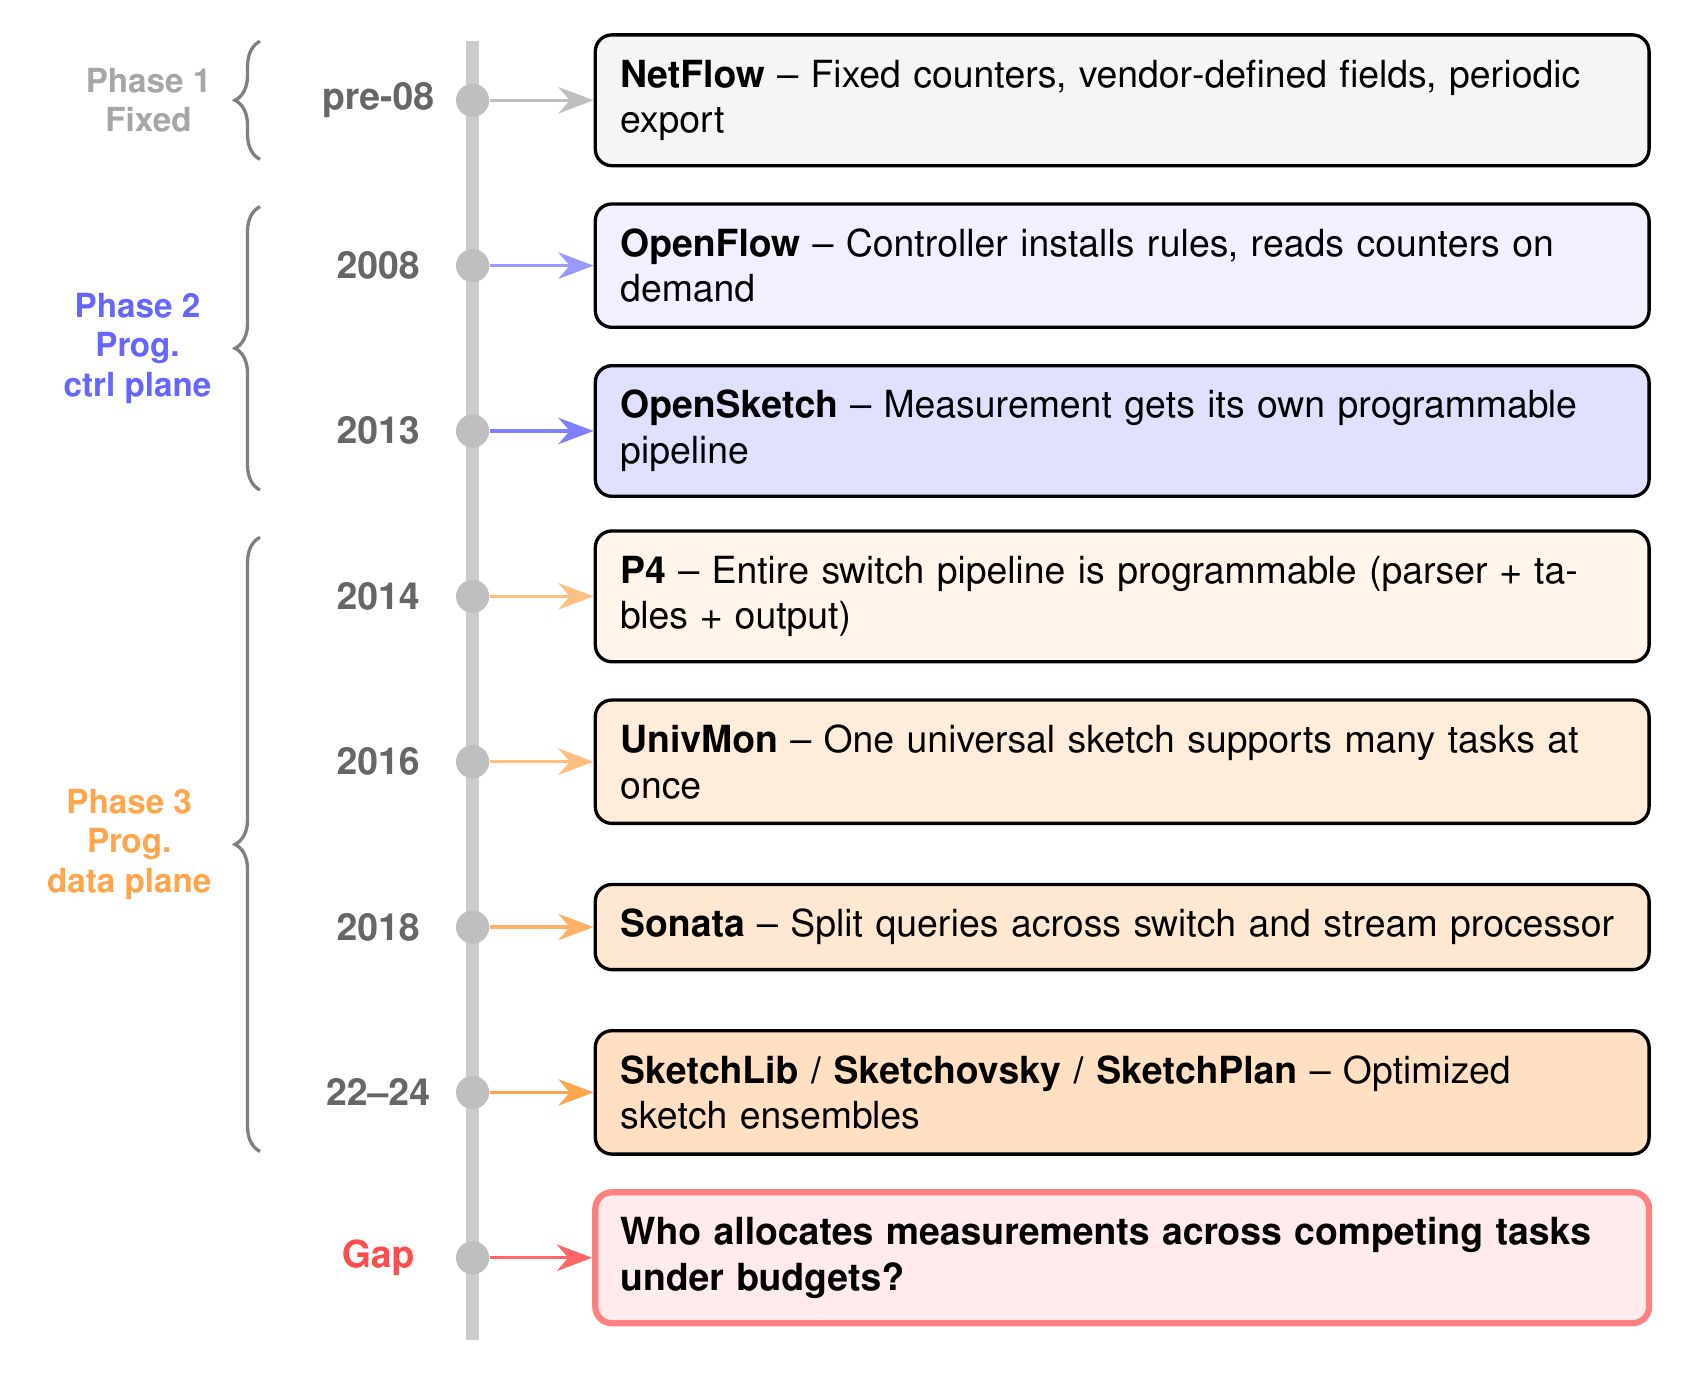
\includegraphics[width=\columnwidth]{fig1_timeline.png}
  \caption{Three phases of network monitoring. Phase~1 offered
    fixed measurement. Phase~2 made the control plane programmable.
    Phase~3 made the data plane programmable. The gap at the
    bottom---deciding which measurements to run under competing
    demands---is what this paper addresses.}
  \label{fig:timeline}
\end{figure}

\subsection{Phase 1: Fixed monitoring (pre-2008)}

Before SDN, network devices came with built-in counters and
sampling mechanisms that the operator could turn on or off but
could not fundamentally change.
NetFlow~\cite{claise2004netflow}, introduced by Cisco in the
1990s, is the best-known example. It recorded per-flow
statistics---source and destination addresses, port numbers,
protocol type, packet counts, byte counts---and exported them
periodically to a collector. The operator could configure how
often to export and what sampling rate to use, but the set of
fields the router could observe was fixed in silicon. If an
operator wanted to track a metric that NetFlow did not support
(say, per-packet latency or entropy of destination addresses),
there was no way to do it without replacing the hardware.

This rigidity was a direct consequence of the hardware design
philosophy of the era: every protocol and every measurement
function was burned into the chip at manufacturing time.

\subsection{Phase 2: Programmable control plane (2008--2013)}

OpenFlow~\cite{mckeown2008openflow} introduced a different model.
Instead of each switch making its own forwarding decisions based
on built-in logic, a central controller installed rules into the
switch's flow table over a secure channel. Each rule said: ``if a
packet matches this pattern, do this action (forward to port X,
drop, send to controller).'' Crucially, each rule also had
counters that recorded how many packets and bytes had matched it.

This gave monitoring two new capabilities that NetFlow lacked.
First, the controller could install rules \emph{specifically}
for measurement purposes---rules whose only job was to match a
set of flows and count them. Second, the controller could change
those rules at any time, adding new ones when suspicious traffic
appeared and removing old ones when they were no longer needed.
Monitoring became dynamic rather than static.

But OpenFlow switches were still limited in what they could do
with each packet. They could match on header fields and count
matches, but they could not run more complex operations. A switch
could tell you how many packets matched rule~42, but it could not
compute a hash of the source address, update a probabilistic
counter, or embed a timestamp into the packet header. For
anything beyond simple counting, the data had to be sent to the
controller or a separate collector for processing.

OpenSketch~\cite{yu2013opensketch} was one of the first systems
to recognize that measurement needed its own programmable
pipeline, separate from forwarding. It proposed a three-stage
architecture---hash, filter, count---implemented on NetFPGA
hardware, with a control-plane library that automatically
configured the pipeline for different measurement tasks (heavy
hitter detection, change detection, flow size estimation). The
key insight was that measurement is itself a resource allocation
problem: different tasks need different amounts of memory and
computation, and the system must decide how to divide limited
hardware resources among them. This idea is a direct ancestor
of the work we propose.

\subsection{Phase 3: Programmable data plane (2014--present)}

P4~\cite{bosshart2014p4} generalized OpenSketch's insight from
measurement to the entire switch pipeline. Where OpenSketch
provided a fixed three-stage pipeline for measurement, P4 made
everything programmable: how the switch parses incoming packets
(which headers to extract), how it matches them (which fields to
compare against which tables), and what actions to take (forward,
drop, modify headers, update state). A programmer writes a P4
program that defines all of this, compiles it, and loads it onto
the switch hardware.

For monitoring, this was transformative. A P4 program can define
custom data structures called \emph{sketches}---compact arrays
that use hash functions to map packet fields to counters, allowing
approximate but memory-efficient tracking of traffic statistics.
It can implement \emph{in-band network telemetry} (INT), where
each switch appends a small metadata header to selected packets
as they pass through, recording queue depth, processing latency,
and other per-hop information. And it can do all of this at line
rate---billions of packets per second---because the logic runs in
the switch's forwarding pipeline, not on a general-purpose CPU.

This phase produced a rapid series of advances in what the switch
can do for measurement.

UnivMon~\cite{liu2016univmon} showed that a single ``universal
sketch'' can support many different monitoring tasks (heavy
hitters, entropy estimation, flow size distribution, change
detection) with accuracy comparable to custom per-task algorithms.
The key idea is that instead of running a separate sketch for
each task, you run one general-purpose sketch and compute
different estimates from it at query time. UnivMon demonstrated a
P4 implementation and a control plane that coordinates sketches
across multiple switches.

Sonata~\cite{gupta2018sonata} introduced query-driven telemetry.
Operators write monitoring queries in a high-level language (``find
all hosts with more than 100 new TCP connections in the last
minute''), and the system automatically decides how much of each
query to run on the switch (at line rate) and how much to send
to a stream processor (which is slower but more flexible). This
partitioning reduced stream-processor load by up to seven orders
of magnitude.

SketchLib~\cite{namkung2022sketchlib} analyzed why sketches are
often infeasible on real switch hardware even though they work
fine in simulation. The problem is that hardware switches have
specific constraints---limited stateful ALUs (arithmetic logic
units that can update counters), limited hash units, and a fixed
number of pipeline stages---and naive sketch implementations
waste these resources. SketchLib identified five categories of
bottlenecks and provided optimization techniques that cut
resource usage by up to 96\%.

Sketchovsky~\cite{namkung2023sketchovsky} extended this to
\emph{ensembles} of sketches. A network operator who needs to
track heavy hitters, estimate flow entropy, and detect
superspreaders simultaneously would normally need three separate
sketches, each consuming its own hash units, counters, and
pipeline stages. Sketchovsky showed that these sketches can share
resources---reuse hash computations, merge counter arrays, share
key-field extraction---making ensembles of up to 18 sketch
instances feasible on a single Tofino switch where only a few
would fit without sharing.

HeteroSketch~\cite{agarwal2022heterosketch} tackled the
network-wide version of this problem: given a network of switches
with \emph{different} capabilities (some programmable, some
fixed-function, some with more memory than others), how do you
decide which device runs which measurement task? Its
profiling-based optimizer matched tasks to device capabilities and
reduced resource overhead by 20--60\%.

SketchPlan~\cite{srivastava2024sketchplan} raised the
abstraction further. Instead of asking operators to choose
specific sketches and configure their parameters, SketchPlan lets
them specify measurement \emph{intents}: ``I want heavy-hitter
detection with 95\% recall and 3\% relative error.'' The system
automatically selects the right sketches, configures them, and
takes an ensemble view that jointly optimizes across multiple
intents. This improved accuracy--resource tradeoffs by up to
60$\times$ compared to optimizing each intent in isolation.

OctoSketch~\cite{zhang2024octosketch} addressed a different
bottleneck: software switches that process packets across
multiple CPU cores. Merging sketch results from different cores
introduces errors and computation overhead. OctoSketch devised a
continuous, change-based aggregation mechanism that reduced errors
by 15.6$\times$ and improved throughput by up to 4.5$\times$.

\subsection{What is still missing}

Each of these systems solves one piece of the puzzle. The sketch
papers tell us \emph{how} to run measurements efficiently on
hardware. The polling papers tell us \emph{when} to collect
statistics. The placement papers tell us \emph{where} in the
network to put monitors. But nobody answers the combined
question: given a fixed budget of switch memory, controller CPU,
and bandwidth, and given multiple applications that all want
measurements at the same time, \emph{which measurements should
actually run?}

\Cref{fig:coverage} makes this gap concrete. It maps eleven
systems against five decision dimensions. No prior system covers
more than two.

\begin{figure}[t]
  \centering
  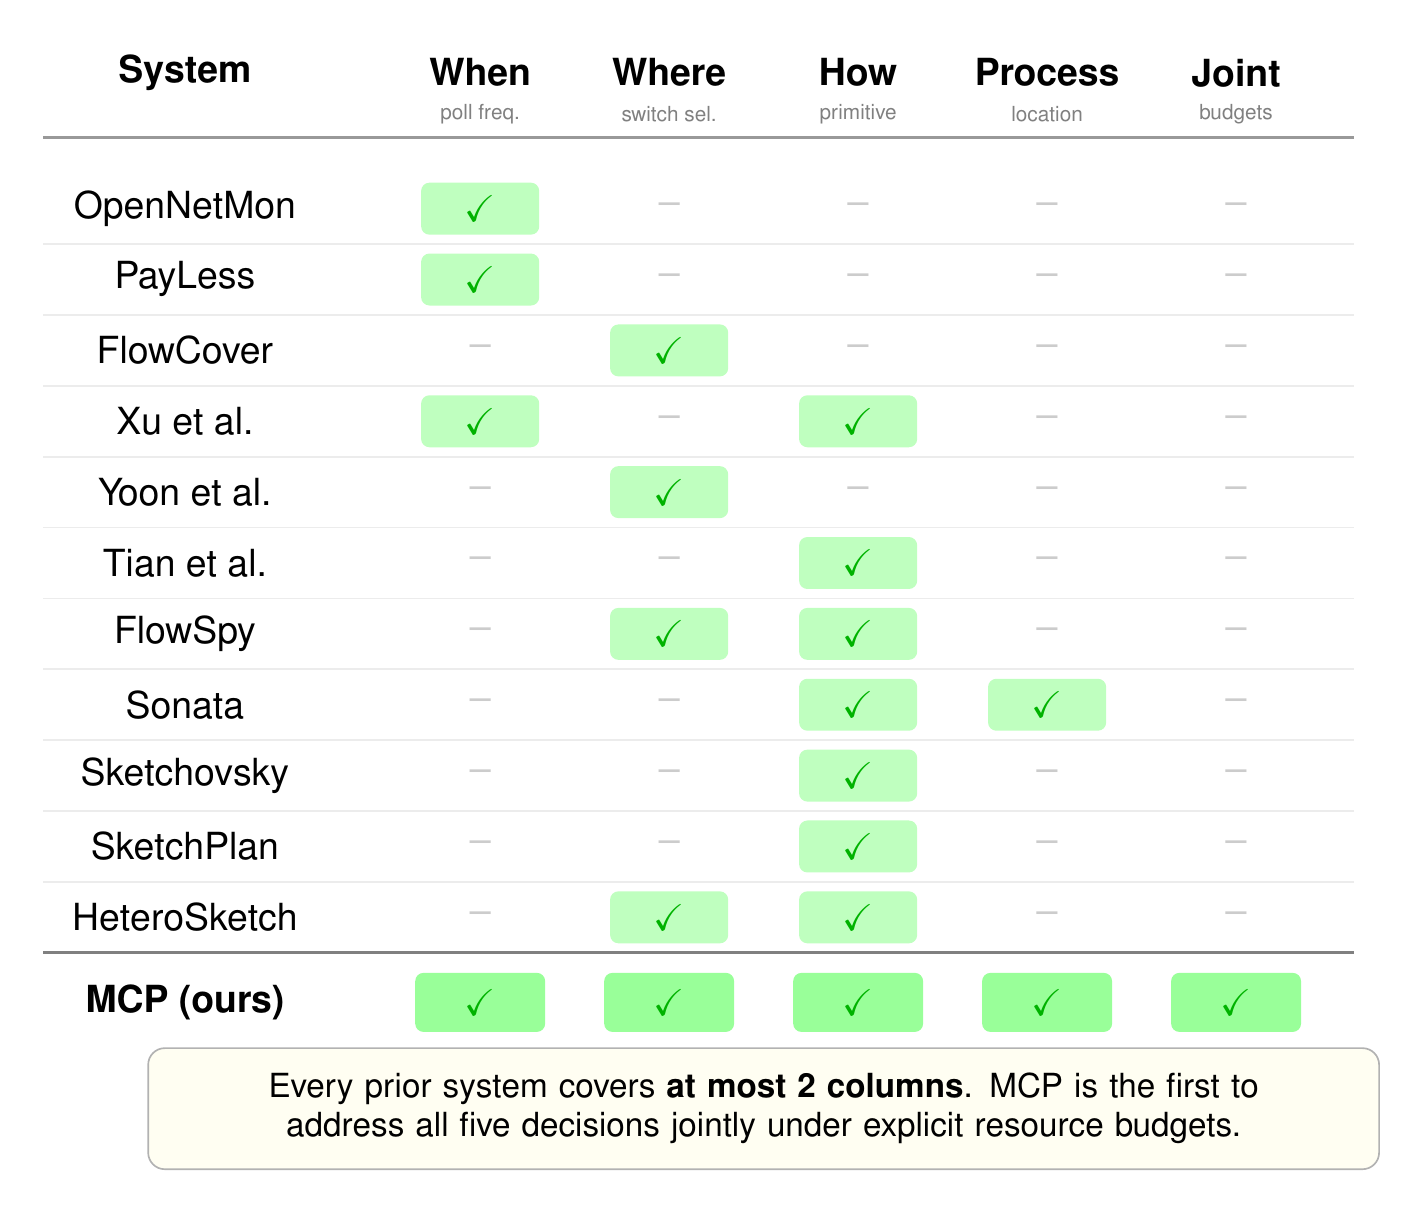
\includegraphics[width=\columnwidth]{fig2_coverage.png}
  \caption{What each system decides. \emph{When} = polling
    frequency. \emph{Where} = which switches. \emph{How} =
    which primitive (counter, sketch, sample, INT).
    \emph{Process} = where to compute (switch vs.\ controller
    vs.\ stream processor). \emph{Joint} = multi-objective
    allocation under budgets. Every prior system covers at most
    two columns. \system covers all five.}
  \label{fig:coverage}
\end{figure}

%----------------------------------------------------------------------
\section{What the Literature Got Right---and Where It Disagrees}
\label{sec:landscape}

We analyzed eighteen systems spanning 2008--2024 and organized
them not by publication date but by what they optimize and what
they assume.

\subsection{What the field agrees on}

Four claims are supported across the entire corpus.

First, \textbf{brute-force monitoring does not scale.} Polling
every counter at high frequency floods the control channel with
request-response messages. Installing a measurement rule for
every individual flow exhausts the TCAM (Ternary Content-Addressable
Memory), which is the scarce, power-hungry memory that stores
matching rules inside the switch. Every paper in this corpus
either demonstrates or assumes this constraint.

Second, \textbf{being selective helps.} Whether by adapting
polling intervals so that stable flows are checked less
often~\cite{adrichem2014opennetmon, chowdhury2014payless},
choosing which switches to poll~\cite{su2014flowcover}, picking
only measurements that add new information to a traffic-matrix
estimate~\cite{tian2018trafficmatrix}, or selecting sampling
points by betweenness centrality~\cite{yoon2017sampling}, the
field agrees that targeted monitoring outperforms exhaustive
monitoring.

Third, \textbf{the value of a measurement depends on the task.}
A per-flow byte counter is useful for QoS monitoring but
irrelevant for DDoS detection, which cares more about the number
of distinct source addresses per destination. A traffic-matrix
estimator needs measurements that are linearly independent from
measurements already taken, while an IDS needs measurements from
switches that see the widest variety of traffic. Different tasks
need fundamentally different measurement strategies.

Fourth, \textbf{programmability changes everything.} Each
generation of programmability---OpenFlow (programmable control
plane), OpenSketch (programmable measurement pipeline), P4
(programmable data plane)---opened new ways to measure. The latest
generation (P4 with sketch libraries) makes it physically possible
to run many measurement tasks on one switch, but this creates a
new allocation problem: which tasks get which resources?

\subsection{Three research directions}

The eighteen systems cluster into three directions.

\para{Direction 1: Make polling cheaper}
OpenNetMon~\cite{adrichem2014opennetmon} and
PayLess~\cite{chowdhury2014payless} adapt polling frequency:
poll more often when traffic changes rapidly, less often when it
is stable. Xu~\etal\cite{xu2017wildcard} reduce the number of
requests by using wildcard rules that aggregate multiple flows
into a single counter, cutting both control-channel bandwidth and
switch processing delay.

\para{Direction 2: Choose better measurement targets}
FlowCover~\cite{su2014flowcover} picks which switches to poll
using a weighted set-cover optimization.
Tian~\etal\cite{tian2018trafficmatrix} pick which flows to
measure based on whether each new measurement increases the rank
of the traffic-matrix estimation system---if it does not, the
measurement is redundant and wastes a TCAM entry.
FlowSpy~\cite{guan2019flowspy} assigns monitoring tasks to P4
switches with explicit load balancing.
HeteroSketch~\cite{agarwal2022heterosketch} places sketches
across heterogeneous devices by profiling each device's
capabilities first.
Tahaei~\etal\cite{tahaei2018distributed} redesign measurement
for the practical reality of distributed controllers, where
synchronization overhead becomes a first-class cost.

\para{Direction 3: Make the switch pipeline do more}
This direction, described in \cref{sec:background}, includes
OpenSketch~\cite{yu2013opensketch},
UnivMon~\cite{liu2016univmon},
Sonata~\cite{gupta2018sonata},
SketchLib~\cite{namkung2022sketchlib},
Sketchovsky~\cite{namkung2023sketchovsky},
SketchPlan~\cite{srivastava2024sketchplan}, and
OctoSketch~\cite{zhang2024octosketch}.
For security, Yoon~\etal\cite{yoon2017sampling} choose sampling
points by centrality, and
El~Sayed~\etal\cite{elsayed2022ddos} build SDN-native DDoS
classifiers using features extracted from flow statistics.

\subsection{Assumptions nobody tests}
\label{sec:assumptions}

We found six assumptions that most papers rely on without
experimental validation.

\para{A1: Switch counters are accurate enough to optimize around}
All polling-based systems use switch-reported counters as ground
truth for their optimization decisions. But switch counters can
be stale (updated at different rates than the polling interval),
delayed (buffered before export), or affected by internal
scheduling artifacts. If the counters are noisy at timescales
that matter for the optimization, the cost--accuracy tradeoffs
these papers report may not hold in practice.

\para{A2: The cost--accuracy tradeoff is smooth}
The literature implicitly assumes that if you reduce measurement
(poll less often, use fewer rules, run smaller sketches), accuracy
degrades gradually and predictably. But if the tradeoff has
discontinuities---sharp cliffs where a small reduction in
measurement causes a large drop in visibility---then the smooth
tradeoff curves in these papers overstate the practical operating
range.

\para{A3: Partial observation catches what matters}
Selective monitoring works only if the ``right'' subset of flows
to observe does not change faster than the system can adapt its
selection. If an attack appears on a flow that the system decided
not to monitor, partial observation misses exactly what it was
designed to catch.

\para{A4: The controller has spare capacity for monitoring}
Even systems that reduce polling overhead assume the controller
can absorb the remaining monitoring workload without affecting
its primary job of managing forwarding rules. If monitoring and
control compete for the same CPU and memory on the controller
machine, monitoring overhead becomes a control-plane stability
risk.

\para{A5: Lab results transfer to production}
Most evaluations use Mininet (a software emulator) with small
topologies and synthetic traffic.
SketchLib~\cite{namkung2022sketchlib} showed that sketch
implementation details---the specific way hash functions are
assigned to hardware units, how counter widths interact with
stateful ALU constraints---materially change accuracy on real
Tofino hardware compared to software simulation. This is a direct
warning that lab results may not predict deployment behavior.

\para{A6: Better measurement means better network outcomes}
This is the most consequential assumption. Almost every paper in
this corpus stops at measurement quality: lower polling cost,
higher estimation accuracy, better detection rates. None of them
closes the loop to show that the downstream application---the
traffic engineering controller that reroutes flows, the IDS that
blocks attackers, the QoS manager that adjusts
priorities---actually makes better decisions as a result of the
improved monitoring. It is entirely possible that a monitoring
system with excellent internal metrics produces telemetry that the
downstream application cannot use effectively.

%----------------------------------------------------------------------
\section{Where the Papers Contradict Each Other}
\label{sec:contradictions}

Not every difference between systems is a disagreement. Many
papers simply study different problems. But four differences are
genuine contradictions---positions that cannot both be true in
the same deployment.

\para{Contradiction 1: Where should monitoring logic live?}
The OpenFlow-era papers~\cite{adrichem2014opennetmon,
chowdhury2014payless, su2014flowcover} place monitoring
intelligence in the controller. The controller decides what to
measure, sends requests to the switch, collects responses, and
processes the results. The switch is passive---it counts when
asked.
FlowSpy~\cite{guan2019flowspy} and the sketch
papers~\cite{namkung2023sketchovsky} take the opposite position:
monitoring tasks should run directly in the P4 switch pipeline,
with the controller involved only for task assignment, not for
data collection.
El~Sayed~\etal\cite{elsayed2022ddos} take a third position:
detection should stay at the controller because putting
decision-making logic in the switch violates SDN's principle of
separating forwarding from control.

These three positions cannot all be correct for the same network.
The disagreement exists because each group assumed different
hardware. The OpenFlow papers assumed switches that can only
count packets. The P4 papers assumed switches that can run
arbitrary programs. El~Sayed~\etal assumed OpenFlow-era switches
where in-switch intelligence is not feasible. The contradiction
is not about philosophy---it is about which hardware generation
the authors had in mind.

\para{Contradiction 2: Where in the network should monitors sit?}
OpenNetMon monitors at edge switches because they sit at flow
endpoints, making per-flow measurement straightforward.
Yoon~\etal~\cite{yoon2017sampling} monitor at high-centrality
switches because those switches see the most diverse traffic,
which is better for feeding an IDS.
HeteroSketch~\cite{agarwal2022heterosketch} says the answer
depends on each device's hardware capabilities, not just its
topological position.

None of these papers considers what happens when QoS monitoring
(which favors edge switches) and security monitoring (which
favors high-centrality switches) must both run on the same
network with the same set of switches.

\para{Contradiction 3: Does measuring more always help?}
PayLess assumes that finer-grained, higher-frequency collection
improves monitoring quality. This is true for operational
monitoring, where more data generally means more accurate
statistics.
Tian~\etal\cite{tian2018trafficmatrix} explicitly reject this for
traffic-matrix estimation: a measurement that does not increase
the rank of the linear system that maps observable flows to the
full traffic matrix contributes zero new information. Installing
it wastes a TCAM entry that could have been used for a
measurement that actually adds something.

This is not a minor disagreement. It reflects fundamentally
different mathematical structures: operational monitoring has
diminishing returns (more data helps, but with decreasing
marginal benefit), while inverse estimation has a rank
condition (some measurements are completely redundant regardless
of how many you already have).

\para{Contradiction 4: Is a single controller enough?}
The early papers assume a single logically centralized controller
is both sufficient and beneficial---it provides a global view
that makes monitoring easier to orchestrate.
Tahaei~\etal\cite{tahaei2018distributed} argue that in practice,
a single physical controller creates scalability, reliability,
and performance bottlenecks.
El~Sayed~\etal\cite{elsayed2022ddos} go further: even multiple
controllers do not help for DDoS defense, because the
controllers themselves can be targeted by the attack.

\para{What these contradictions mean for \system}
Each system picks one objective, designs an architecture that
serves it well, and treats the other objectives as someone else's
problem. A deployed network has QoS monitoring, traffic
estimation, attack detection, and more, all running at the same
time on the same hardware. The contradictions arise because
nobody has built the layer that manages these competing demands.
That is the gap \system addresses.

%----------------------------------------------------------------------
\section{Proposed Design: A Measurement Control Plane}
\label{sec:design}

\system is a subsystem that \textbf{lives in the control plane},
alongside the forwarding controller. It does not run on any
switch. It reads switch state over standard interfaces, makes
allocation decisions on general-purpose hardware, and writes
measurement configurations back to switches.
\Cref{fig:topology} shows exactly where it sits.

\begin{figure*}[t]
  \centering
  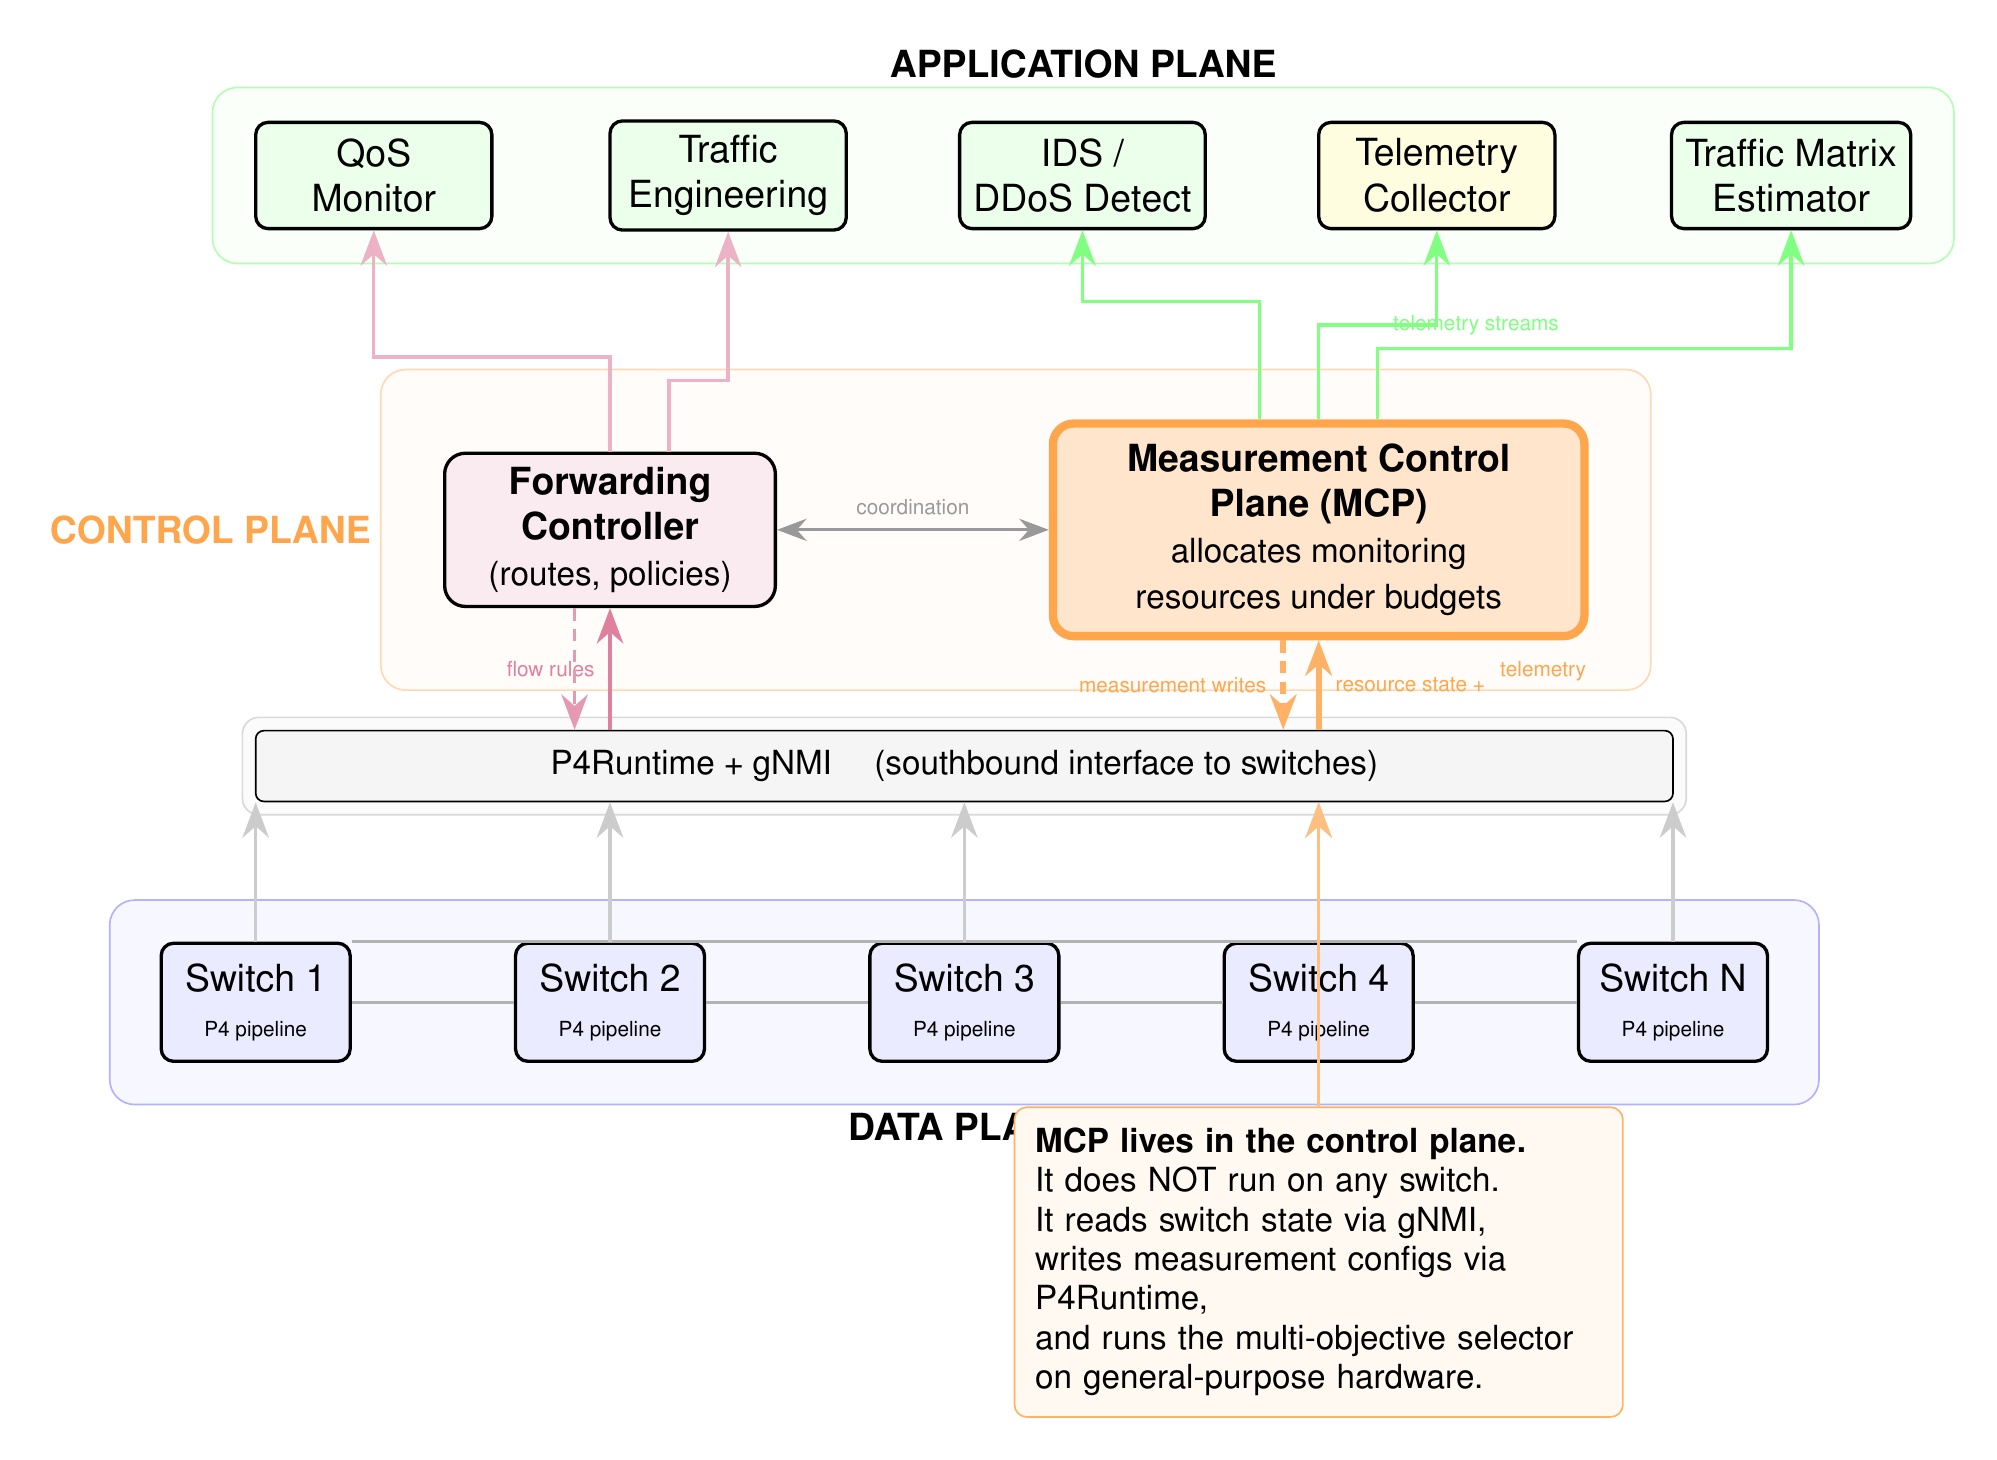
\includegraphics[width=\textwidth]{fig3_topology.png}
  \caption{Where \system lives in the network. \system sits in
    the \textbf{control plane}, alongside the forwarding
    controller. It is not part of any switch. It reads switch
    resource state via gNMI (a standard telemetry streaming
    protocol), makes allocation decisions on general-purpose
    hardware, and writes measurement configurations to switches
    via P4Runtime (a standard switch programming API). The
    forwarding controller handles routing and policies; \system
    handles measurement. They coordinate but are separate
    services.}
  \label{fig:topology}
\end{figure*}

\subsection{Why the switch itself is the bottleneck}

To understand why measurement allocation is hard, consider what
happens inside a P4 switch. \Cref{fig:pipeline} shows the key
resources.

\begin{figure*}[t]
  \centering
  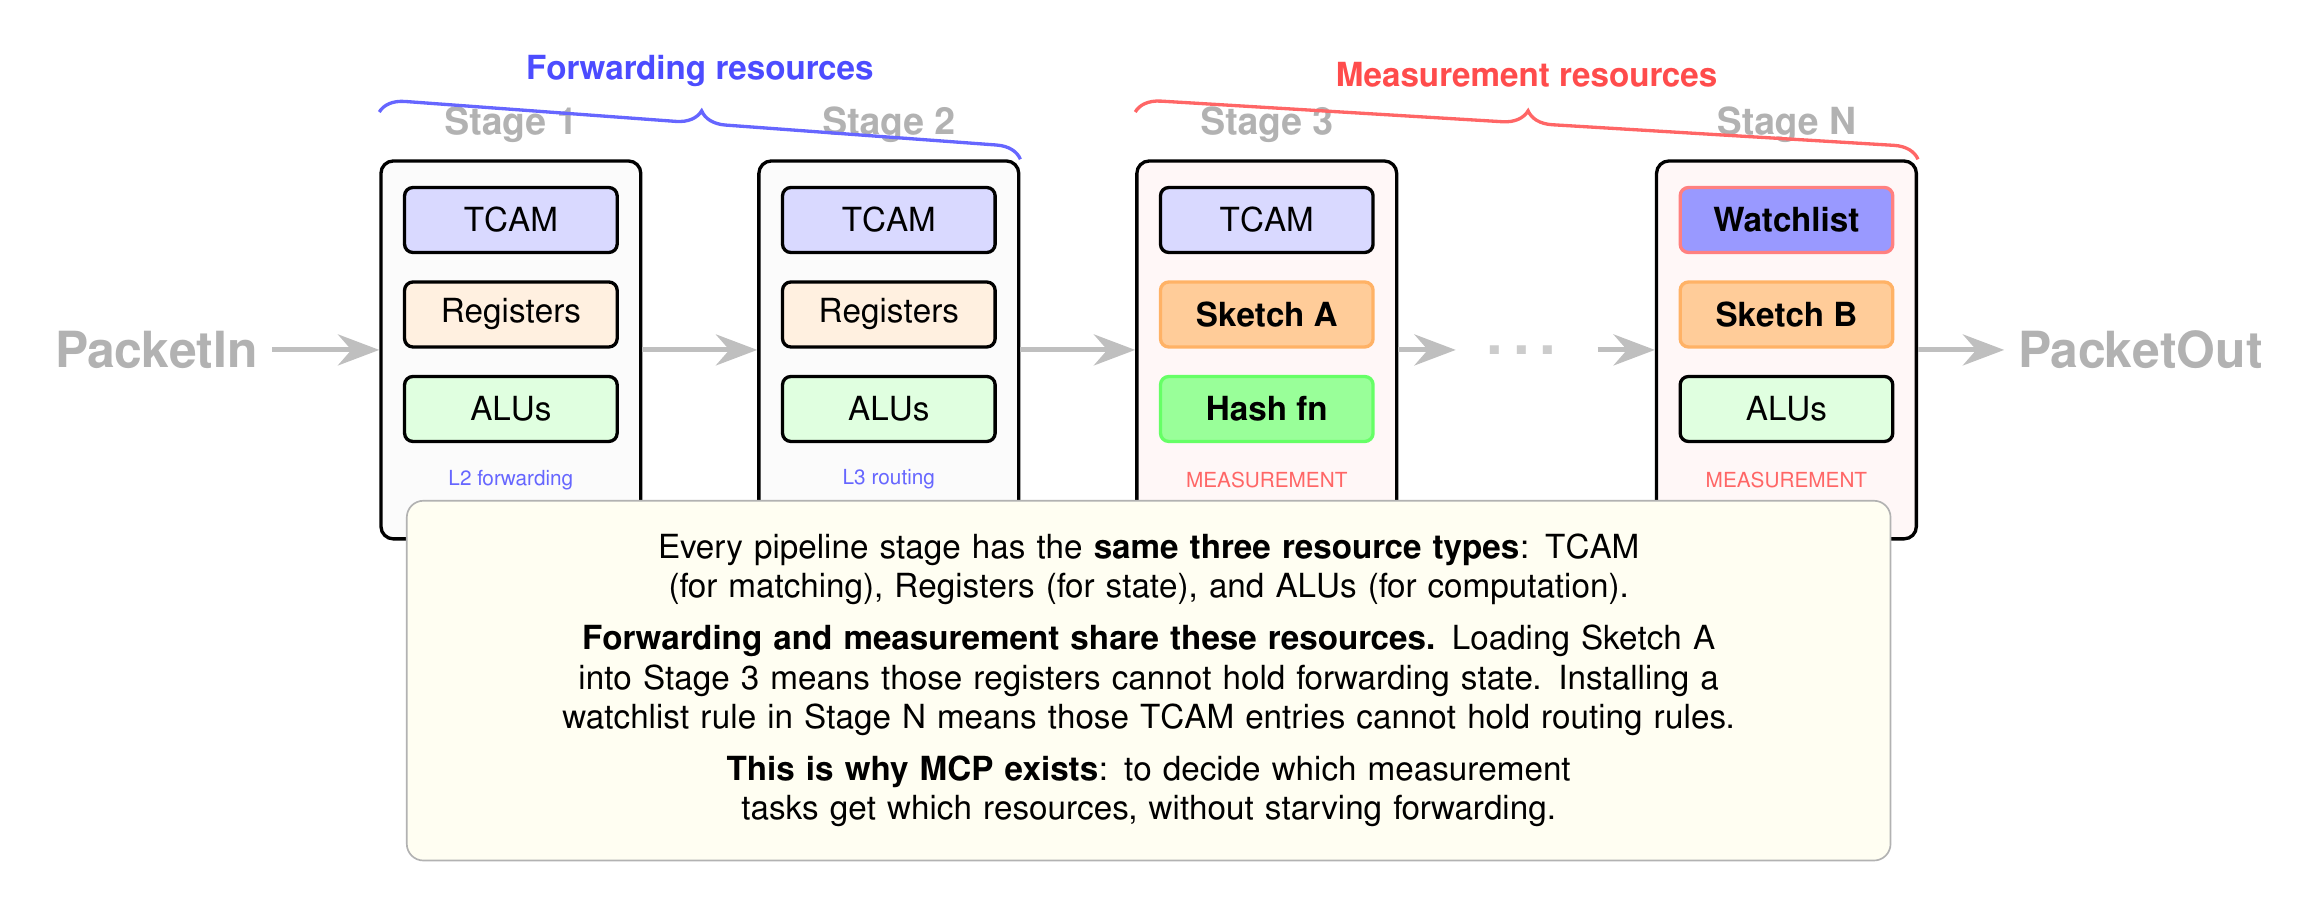
\includegraphics[width=\textwidth]{fig4_pipeline.png}
  \caption{Inside a P4 switch pipeline. Packets flow left to
    right through a series of stages. Each stage has three
    resource types: \textbf{TCAM} (for matching packet headers
    against rules), \textbf{Registers} (for storing state like
    sketch counters), and \textbf{ALUs} (for computation like
    hash functions). Stages~1--2 are used for forwarding (blue
    annotation). Stages~3 and~N show measurement tasks loaded
    by \system (red annotation): a sketch array, a hash
    function, and a watchlist rule. These consume the same
    physical resources that forwarding uses. This is why
    measurement allocation is a resource competition, not just
    a design choice.}
  \label{fig:pipeline}
\end{figure*}

A P4 switch processes packets through a series of \emph{pipeline
stages}. Each stage is a self-contained hardware block that can
match on packet headers and perform actions. The number of stages
is fixed at chip fabrication---a typical Tofino switch has 12
ingress stages and 12 egress stages. You cannot add more.

Within each stage, three types of resources are available.
\textbf{TCAM} (Ternary Content-Addressable Memory) stores
matching rules. A forwarding rule (``if destination IP matches
10.0.0.0/24, send to port~3'') uses TCAM entries. A measurement
watchlist rule (``if source IP is in the suspicious set, increment
a counter'') also uses TCAM entries. Both compete for the same
finite memory.
\textbf{Registers} store persistent state. A forwarding
application might use registers to track connection state. A
sketch data structure uses register arrays to store approximate
counters. Both compete for the same on-chip SRAM.
\textbf{ALUs} (Arithmetic Logic Units) perform computation.
Forwarding logic might use an ALU to compute an ECMP hash for
load balancing. A sketch uses ALUs to compute hash functions for
updating counters. Both compete for the same hardware units.

When \system loads a sketch array into Stage~3, those registers
are no longer available for forwarding state. When it installs a
watchlist rule in Stage~N, those TCAM entries are no longer
available for routing rules. This is why measurement allocation
is a resource problem, not just a configuration choice: every
measurement task takes a piece of the fixed pipeline, and the
pipeline cannot grow.

\subsection{Architecture overview}

\system has three layers, shown in \cref{fig:topology}.

\para{Layer 1: Data plane (the switches)}
Each P4 switch runs measurement primitives: sketch arrays,
per-flow counters, sampling/mirroring with meter-based rate caps,
and optional INT headers. These are compiled into the switch
pipeline using the Portable Switch Architecture
(PSA)~\cite{p4psa}. The switch reports its current resource
usage---how many TCAM entries are in use, how much register
memory is allocated, which pipeline stages are committed---to
\system via gNMI (gRPC Network Management Interface), a standard
protocol for streaming device telemetry.

\para{Layer 2: Measurement Control Plane (the brain)}
This is the core of the system. It runs on general-purpose
hardware in the control plane---the same server rack or cluster
where the forwarding controller runs. It has four components that
execute in sequence every epoch (a configurable interval;
1~second is a reasonable starting point):

A \emph{context monitor} reads the current network state via gNMI
streams: the traffic mix (how many large flows vs.\ small flows,
the rate of new flow arrivals, which prefixes are most active),
security signals (anomaly scores from the IDS, alert flags from
upstream sensors), topology information (which switches are
connected to which, betweenness centrality values), and resource
utilization (current TCAM occupancy, register usage, controller
CPU load, control-channel bandwidth consumption).

A \emph{candidate generator} produces a bounded list of possible
measurement actions. Each action is a four-part tuple: (1)~what
to observe (a prefix, a 5-tuple class, a set of suspicious
flows), (2)~which primitive to use (counter, sketch, sampled
packets, INT metadata), (3)~at what rate (polling interval,
sampling probability, trigger threshold), and (4)~where to
process the result (on-switch, at the controller, or in a
stream processor). The generator draws on techniques from the
whole literature: set-cover placement from
FlowCover~\cite{su2014flowcover}, wildcard aggregation from
Xu~\etal\cite{xu2017wildcard}, centrality-based sampling from
Yoon~\etal\cite{yoon2017sampling}, sketch ensemble
configuration from
Sketchovsky~\cite{namkung2023sketchovsky}, and query
partitioning from Sonata~\cite{gupta2018sonata}. \system's
contribution is not another measurement technique. It is the
allocator that picks among existing techniques.

A \emph{multi-objective selector} chooses which actions to deploy.
This is where the optimization happens. Every epoch, it
maximizes:
\begin{equation}
  \label{eq:utility}
  U(S_t) = w_{\text{acc}} \cdot \text{Acc}_t
    - w_{\text{lat}} \cdot \text{Lat}_t
    - w_{\text{chg}} \cdot \text{Churn}(S_t, S_{t-1})
\end{equation}
subject to hard budget constraints:
\begin{equation}
  \label{eq:constraints}
  \text{BW}_t \leq \overline{B},\;
  \text{TCAM}_t \leq \overline{T},\;
  \text{REG}_t \leq \overline{R},\;
  \text{CPU}_t \leq \overline{C}
\end{equation}

In plain language: maximize the accuracy of all monitoring tasks
and minimize detection latency, while penalizing frequent
reconfiguration (which disrupts measurement continuity), and
never exceed the operator-specified limits on control-channel
bandwidth, TCAM entries, register memory, or CPU usage. The
weights $w_{\text{acc}}$, $w_{\text{lat}}$, $w_{\text{chg}}$ let
operators express priorities: a security-first deployment would
increase $w_{\text{lat}}$; a bandwidth-constrained deployment
would keep tighter $\overline{B}$.

A \emph{deployer} translates the selected measurement plan into
P4Runtime table writes, register parameter updates, meter
configurations, and gNMI subscription changes. It uses atomic
plan versioning: either the entire plan deploys successfully, or
it rolls back to the previous plan. This prevents partial
configurations where some switches have the new plan and others
still run the old one.

\para{Layer 3: Analytics and actuation}
A collector ingests telemetry reports, packet digests, and
sampled packets from the switches. A stream processor merges
sketch results, computes QoS features, estimates traffic
matrices, and runs IDS inference. An actuator applies mitigation
actions---rate limiting, blackholing, rerouting---when the
analytics layer detects a problem. Outcomes (did detection
latency improve? did the false positive rate change? was the
attack contained?) feed back to the selector as reward signals.

\subsection{How the selector adapts: shadow prices}

The selector uses a type of online learning algorithm called a
\emph{constrained contextual bandit}. To understand why, consider
the three properties of \system's allocation problem:

\begin{enumerate}
\item \textbf{It repeats.} Every epoch (every second), \system
  must choose a new measurement plan. Traffic changes, attacks
  start and stop, resource availability shifts. A static plan
  computed once cannot keep up.
\item \textbf{It has multiple hard constraints.} The plan must
  not exceed budgets for TCAM, registers, bandwidth, and CPU.
  These are hard limits, not soft guidelines---exceeding them
  means the switch cannot install the rules or the controller
  crashes.
\item \textbf{The rewards are unknown.} How much accuracy or
  latency improvement a given measurement action provides
  depends on the current traffic, which \system does not know in
  advance. It must learn from experience.
\end{enumerate}

The Bandits with Knapsacks framework~\cite{badanidiyuru2018bwk}
is designed for exactly this situation: online decision-making
with unknown rewards and budget constraints. Recent work by
Foster~\etal\cite{foster2023contextual} extends it to
contextual settings with multiple packing constraints, which
matches \system's multi-budget structure.

The mechanism that makes this work in practice is \emph{shadow
prices}. \Cref{fig:shadow} illustrates the idea.

\begin{figure*}[t]
  \centering
  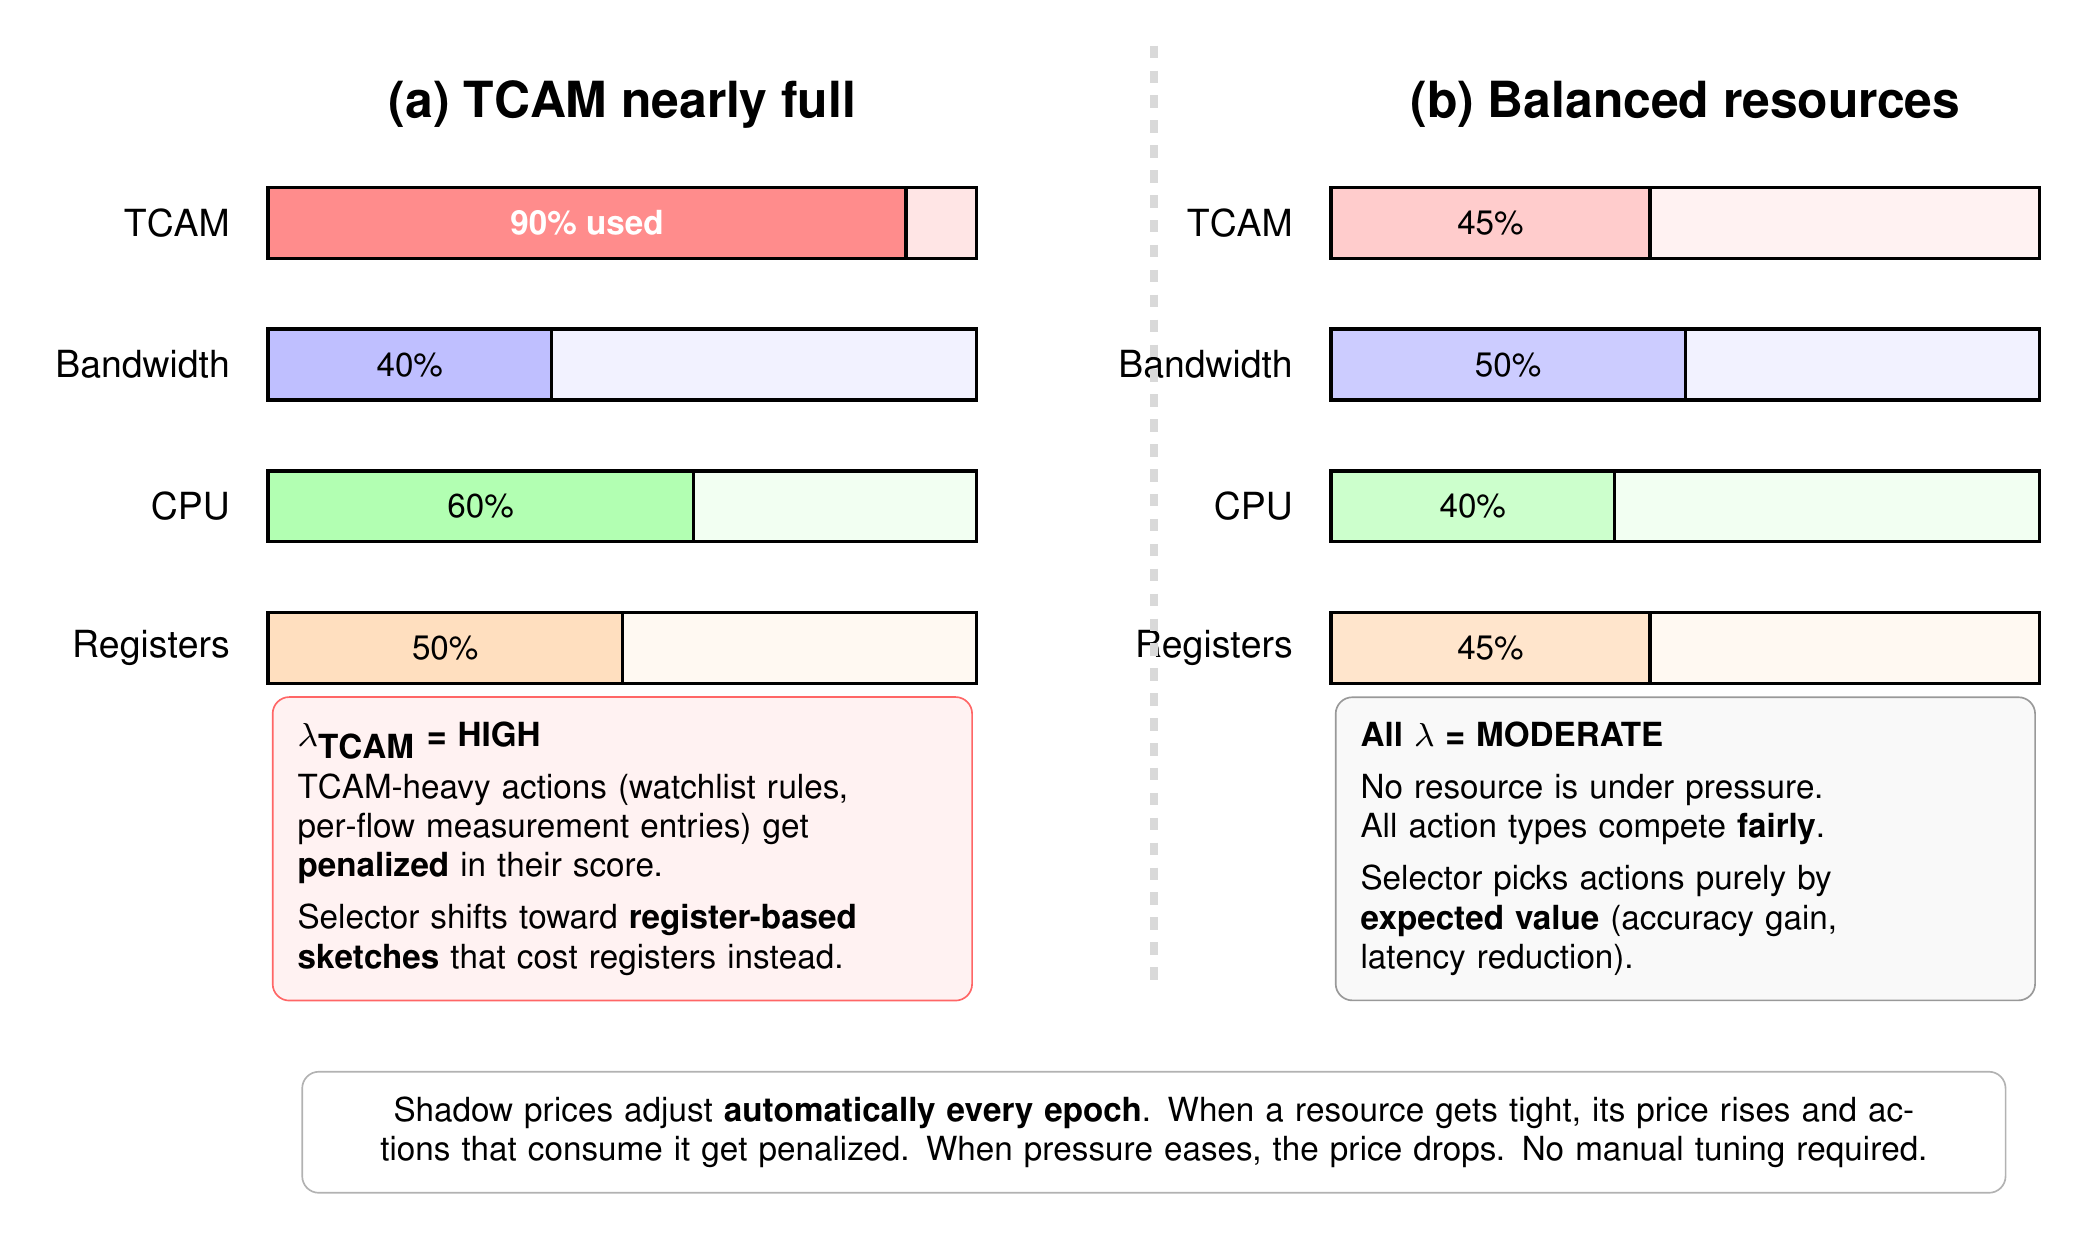
\includegraphics[width=\textwidth]{fig5_shadow.png}
  \caption{How shadow prices steer allocation. (a)~When TCAM is
    90\% full, the shadow price $\lambda_{\text{TCAM}}$ rises
    high, making TCAM-heavy actions (watchlist rules, per-flow
    entries) look expensive in the scoring function. The selector
    shifts toward register-based sketches, which consume registers
    instead of TCAM. (b)~When all resources have headroom, shadow
    prices are moderate and the selector picks actions by expected
    value alone. Shadow prices adjust automatically every epoch.
    No manual rebalancing is needed.}
  \label{fig:shadow}
\end{figure*}

Each resource (TCAM, registers, bandwidth, CPU) has a shadow
price $\lambda_i$ that tracks how tight the budget is. When TCAM
is 90\% full, $\lambda_{\text{TCAM}}$ rises, making any action
that consumes TCAM entries---like installing a watchlist
rule---look expensive in the selector's scoring function. The
selector naturally shifts toward actions that use registers
instead (like sketch arrays). When bandwidth has plenty of
headroom, $\lambda_{\text{BW}}$ drops, making polling-based
actions (which consume bandwidth) look cheap.

This happens automatically every epoch. The update rule is
simple: $\lambda_i \leftarrow \max(0, \lambda_i + \eta \cdot
(\text{realized\_cost}_i - \overline{B}_i))$. If the realized
cost for resource~$i$ exceeds its budget, $\lambda_i$ increases.
If it is below budget, $\lambda_i$ decreases. No operator
intervention is needed.

\Cref{alg:mcprt} gives the full pseudocode.

\begin{algorithm}[t]
  \caption{MCP-RT: Real-time measurement allocation}
  \label{alg:mcprt}
  \begin{algorithmic}[1]
    \REQUIRE Budgets $\overline{B}$; headroom $\rho$;
      value model $V(a|x;\theta)$; cost model $\hat{C}(a|x)$
    \STATE Init shadow prices $\lambda \geq 0$,\;
      $S_{\text{prev}} \leftarrow \emptyset$
    \FOR{each epoch $t$}
      \STATE $x_t \leftarrow$ observe context via gNMI
      \STATE $A_t \leftarrow$ generate candidates
      \FOR{each $a \in A_t$}
        \STATE score$(a) \leftarrow V(a|x_t;\theta)
          - \lambda \cdot \hat{C}(a|x_t)$
      \ENDFOR
      \STATE $R \leftarrow (1{-}\rho)\overline{B}
        - \text{current\_usage}$
      \STATE $S_t \leftarrow \emptyset$;\;
        sort $A_t$ by score/cost descending
      \FOR{each $a$ in sorted order}
        \IF{score$(a) > 0$ \textbf{and} fits$(a, R)$
          \textbf{and} churn\_ok$(a, S_{\text{prev}})$}
          \STATE $S_t \leftarrow S_t \cup \{a\}$;\;
            $R \leftarrow R - \hat{C}(a)$
        \ENDIF
      \ENDFOR
      \STATE Deploy $S_t$ via P4Runtime + gNMI
      \STATE Observe outcomes $y_t$
      \STATE $\theta \leftarrow \text{bandit\_update}(\theta,
        x_t, S_t, \text{reward}(y_t))$
      \STATE $\lambda_i \leftarrow \max(0,\;
        \lambda_i + \eta(\text{cost}_i - \overline{B}_i))$
        \quad $\forall i$
      \STATE $S_{\text{prev}} \leftarrow S_t$
    \ENDFOR
  \end{algorithmic}
\end{algorithm}

\subsection{Why not a simpler approach?}

A natural question is: why not just solve an optimization problem
every epoch, without the bandit machinery? The answer is that the
problem has two features that make static optimization
insufficient. First, several subproblems are NP-hard: the
set-cover placement from FlowCover and the wildcard scheduling
from Xu~\etal both require combinatorial search. Second, the
reward function---how much accuracy or latency improvement each
action actually provides under the current traffic---is unknown.
The bandit learns it from experience.

A second question is: why not full reinforcement learning, which
can handle long-term credit assignment? Because constrained RL
(like CPO~\cite{achiam2017cpo}) is heavier-weight and harder to
safety-engineer for always-on production monitoring. If the RL
agent explores poorly, it could exceed a budget and crash the
switch. The constrained bandit with shadow prices is a practical
middle ground: it learns, it respects budgets by construction,
and it is lightweight enough to run every second.

%----------------------------------------------------------------------
\section{How to Test Whether This Works}
\label{sec:eval}

Testing \system requires going beyond measurement quality.
\Cref{fig:closedloop} shows the full evaluation cycle.

\begin{figure}[t]
  \centering
  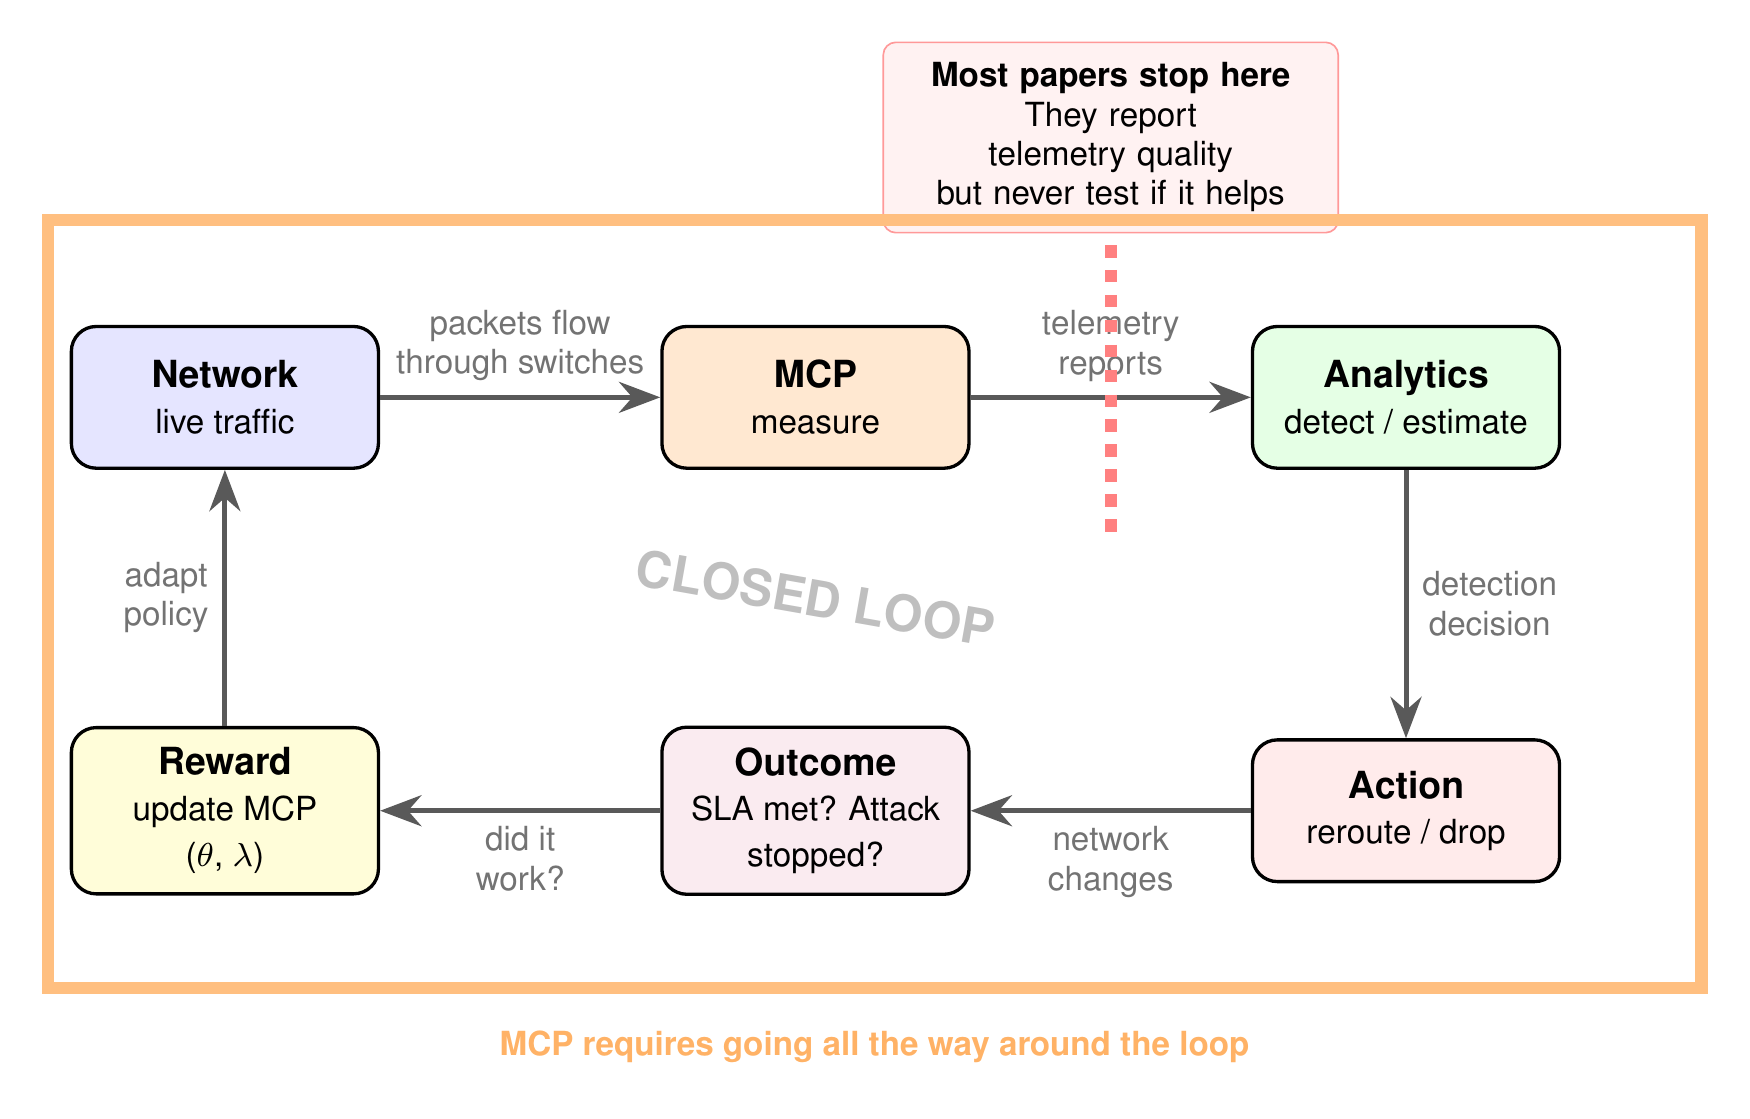
\includegraphics[width=\columnwidth]{fig6_closedloop.png}
  \caption{The closed-loop evaluation cycle that \system requires.
    Most monitoring papers stop at the ``Analytics'' box: they
    report telemetry quality but never test whether the
    downstream application (rerouting, attack blocking) actually
    makes better decisions. \system requires completing the entire
    loop: measuring, analyzing, acting, observing the outcome, and
    feeding the result back to update the measurement policy. Only
    by going all the way around can we test whether better
    monitoring makes the network work better.}
  \label{fig:closedloop}
\end{figure}

\para{Report all objectives simultaneously}
Control-channel bandwidth, switch resource utilization (TCAM
entries, pipeline stages, register memory), controller CPU,
per-task measurement accuracy, and downstream application quality
must all be reported together. A system that improves one metric
while silently degrading another has not made progress---it has
just moved the problem.

\para{Run competing tasks}
At minimum, run QoS estimation and DDoS detection simultaneously
on the same switches. Single-task evaluations completely hide the
allocation problem that \system is designed to solve.

\para{Close the loop}
Connect \system's telemetry output to at least one downstream
application---a traffic engineering controller, a rate limiter,
an alerting system---and measure whether that application's
decisions improve compared to each baseline. If the downstream
application does not improve, the monitoring system's internal
metrics (accuracy, latency, cost) are irrelevant.

\para{Test on real hardware}
At least one experiment must run on a P4 hardware target (Intel
Tofino or equivalent) to confirm that the resource model is
accurate and that measurement primitives operate at line rate
under the proposed allocation.

\para{Baselines}
Each baseline represents one technique from the literature,
running in isolation: (1)~fixed periodic polling, (2)~adaptive
polling~\cite{adrichem2014opennetmon}, (3)~placement-only
optimization~\cite{su2014flowcover}, (4)~wildcard
aggregation~\cite{xu2017wildcard}, (5)~centrality-based
sampling~\cite{yoon2017sampling}, (6)~query-driven partitioning
(Sonata-style~\cite{gupta2018sonata}), (7)~sketch-based
measurement
(Sketchovsky~\cite{namkung2023sketchovsky}), and (8)~fixed-policy
INT. \system should outperform each in multi-objective Pareto
terms, not just on any single metric.

\para{Testbed}
Start with Mininet + Stratum BMv2 + ONOS for toolchain
validation. Move to a Tofino-based hardware switch for
resource-ceiling realism. Use CICIDS2017 and InSDN datasets for
security evaluation, replayed into the SDN fabric with
flow-level labels.

%----------------------------------------------------------------------
\section{What Can Go Wrong}
\label{sec:failures}

\Cref{tab:failures} lists the failure modes we anticipate and the
mitigations designed into the architecture.

\begin{table}[t]
  \caption{Anticipated failure modes and mitigations.}
  \label{tab:failures}
  \centering
  \footnotesize
  \begin{tabular}{@{}p{1.6cm}p{2.2cm}p{2.6cm}@{}}
    \toprule
    Failure & Cause & Mitigation \\
    \midrule
    Telemetry storms &
      INT triggers too broad; incident causes export flood &
      Per-switch meter caps; shadow prices spike for BW;
      shed low-value actions first \\
    \addlinespace
    CPU saturation &
      Excessive polling or feature computation &
      Explicit CPU budget; offload to switch sketches or stream
      processor \\
    \addlinespace
    TCAM exhaustion &
      Measurement rules crowd out forwarding &
      Hard cap; prioritize high-information candidates;
      fall back to register-based sketches \\
    \addlinespace
    Reconfig churn &
      Frequent updates cause oscillation &
      Churn penalty in utility; max updates per epoch;
      plan versioning + rollback \\
    \addlinespace
    Controller split &
      Delayed sync between distributed controllers &
      Raft-backed budget ledger; single-writer P4Runtime
      mastership per switch \\
    \bottomrule
  \end{tabular}
\end{table}

%----------------------------------------------------------------------
\section{Related Work}
\label{sec:related}

We organize related work by the layer of the monitoring stack
each system addresses, and discuss each system's contribution and
limitations in the context of the multi-objective allocation
problem.

\para{The measurement substrate}
The foundation of all work in this paper rests on four systems
that made monitoring progressively more programmable.
NetFlow~\cite{claise2004netflow} established the paradigm of
flow-level measurement with per-flow counters and periodic export,
but its fixed-function design meant operators could not adapt
measurement to changing conditions.
OpenFlow~\cite{mckeown2008openflow} introduced the separation of
control and data planes, allowing a remote controller to install
and read measurement rules dynamically---a step-change in
flexibility, though the switch itself remained a simple
counter.
OpenSketch~\cite{yu2013opensketch} was the first system to argue
that measurement deserves its own programmable pipeline, separate
from forwarding. Its three-stage architecture (hash, filter,
count) on NetFPGA hardware demonstrated that different
measurement tasks could share the same hardware through
software-controlled configuration---a direct precursor to
\system's resource allocation idea.
P4~\cite{bosshart2014p4} generalized this to the entire switch,
making the parser, match-action tables, and output logic all
programmable. This made sketches, INT, and custom telemetry
feasible at line rate, but also created the resource competition
between forwarding and measurement that motivates \system.

\para{Polling optimization}
OpenNetMon~\cite{adrichem2014opennetmon} adaptively adjusts
polling intervals for edge switches, reducing overhead while
maintaining per-flow QoS visibility (throughput, delay, loss).
Its limitation is that it monitors only at edge switches and
optimizes only polling frequency---it does not consider switch
resource usage or alternative measurement primitives.
PayLess~\cite{chowdhury2014payless} provides a controller-side
monitoring middleware with a REST API, adapting polling schedules
based on traffic dynamics. It demonstrates the
accuracy--overhead tradeoff but does not address multi-controller
deployments or data-plane programmability.
Xu~\etal\cite{xu2017wildcard} reduce the number of statistics
requests by aggregating flows into wildcard groups, cutting both
control bandwidth and switch processing delay. Their work
explicitly models request cost as an optimization variable but
does not consider competing monitoring tasks or switch-side
resource limits beyond processing delay.

\para{Placement and selection}
FlowCover~\cite{su2014flowcover} formulates the problem of
choosing which switches to poll as a weighted set-cover problem,
minimizing communication cost while ensuring all flows are
observed. It provides the strongest formal treatment of the
placement problem among the OpenFlow-era papers, but it does not
account for switch-side resource limits, distributed controllers,
or heterogeneous device capabilities.
Tian~\etal\cite{tian2018trafficmatrix} define measurement value
as information gain for traffic-matrix estimation: each
measurement is worth installing only if it increases the rank of
the linear system. This is the sharpest formulation of measurement
value in the corpus, but it applies only to traffic-matrix
estimation, not to security or QoS tasks.
FlowSpy~\cite{guan2019flowspy} moves monitoring task placement
into the P4 data plane with load balancing, bridging the gap
between OpenFlow-era polling and P4-era in-switch monitoring. It
does not address multi-objective allocation or closed-loop
evaluation.
HeteroSketch~\cite{agarwal2022heterosketch} is the first system
to address network-wide sketch placement across heterogeneous
devices, using a profiling tool to quantify each device's
capabilities and an optimization framework to assign tasks. It
reduces resource overhead by 20--60\% and handles dynamic changes.
Its focus is on sketch placement, not on the broader question of
which measurement \emph{type} (sketch vs.\ polling vs.\ sampling
vs.\ INT) to use at each location.
Tahaei~\etal\cite{tahaei2018distributed} address the gap between
single-controller measurement systems and the reality of
distributed-controller SDN, proposing synchronization-aware flow
measurement to control overhead. Their work is the closest to
recognizing that controller architecture constrains monitoring
design, but it does not address P4 programmability or
multi-objective allocation.

\para{Sketch infrastructure}
UnivMon~\cite{liu2016univmon} introduced the idea of a universal
sketch that delays the binding between data-plane computation and
specific monitoring tasks, achieving both generality and
accuracy. It demonstrated a P4 implementation and network-wide
coordination, laying the theoretical and practical groundwork for
all subsequent sketch-based monitoring.
SketchLib~\cite{namkung2022sketchlib} identified the practical
bottlenecks that make sketches infeasible on real hardware and
provided correct-by-construction optimizations. Its key
contribution is showing that implementation details (how hash
functions map to hardware units, how counter widths interact with
ALU constraints) materially affect both feasibility and accuracy.
Sketchovsky~\cite{namkung2023sketchovsky} optimized ensembles of
sketches through cross-instance resource sharing, making it
feasible to run many measurement tasks on one switch. It tested
on a real Tofino switch with forwarding logic co-resident,
demonstrating practical deployment.
OctoSketch~\cite{zhang2024octosketch} solved the multi-core
aggregation problem for software switches, and
SketchPlan~\cite{srivastava2024sketchplan} raised the
abstraction to intent-level planning with ensemble-wide
optimization. These five systems collectively provide the
measurement primitives that \system would allocate. Our
contribution is orthogonal: we address which primitives to run
where, not how to implement them.

\para{Query-driven telemetry}
Sonata~\cite{gupta2018sonata} is the closest prior work to
\system in spirit: it partitions monitoring queries across the
switch and a stream processor, explicitly considering where
computation should happen. \system adopts Sonata's partitioning
idea as one of its candidate-generation strategies but adds three
things Sonata lacks: explicit multi-resource budgets (TCAM,
registers, CPU), competition between multiple monitoring tasks,
and closed-loop evaluation against downstream outcomes.

\para{Security monitoring}
Yoon~\etal\cite{yoon2017sampling} use betweenness centrality to
select sampling switches for feeding an IDS, with controlled
sample rates to avoid overwhelming the IDS capacity. Their work
is specific to IDS feeding and does not consider how security
sampling competes with QoS or estimation tasks for switch
resources.
El~Sayed~\etal\cite{elsayed2022ddos} show that SDN-native
features and deep-learning classification outperform conventional
approaches for DDoS detection, but their system operates entirely
at the controller and does not consider P4-based data-plane
monitoring or resource-constrained deployment.

\para{Online optimization under resource constraints}
Bandits with Knapsacks~\cite{badanidiyuru2018bwk} provides the
theoretical foundation for online learning under budget
constraints, using primal--dual updates to balance exploration
and exploitation while respecting resource limits.
Foster~\etal\cite{foster2023contextual} extend contextual bandits
to settings with multiple packing and covering constraints,
providing the algorithmic template for \system's multi-budget
selector.
CPO~\cite{achiam2017cpo} offers constrained policy optimization
for longer-horizon problems, but its weight and complexity make
it better suited as a later-stage upgrade once the basic \system
pipeline is validated.

%----------------------------------------------------------------------
\section{Limitations}
\label{sec:limitations}

This paper is an analysis and a proposal, not a working system.
\system has not been implemented. The bandit-based selector has
not been evaluated on any concrete instance, and we do not know
whether it converges fast enough for production use. The churn
penalty and epoch duration~$\Delta$ are open design parameters
that require empirical tuning on real traffic.

Our literature analysis covers eighteen papers selected to span
the major architectural positions from 2008 to 2024. It is not
exhaustive. Work in adjacent areas---eBPF-based host monitoring,
SmartNIC offloading, network verification, and INT/PINT protocol
design---may partially address some of the gaps we identify.

The untested assumptions in \cref{sec:assumptions} are identified
by careful reading of the papers, not by running falsification
experiments. We argue they are untested, not necessarily that they
are wrong. Some may hold up under experimental scrutiny; others
may reveal real gaps.

%----------------------------------------------------------------------
\section{Conclusion}
\label{sec:conclusion}

Network monitoring has moved through three phases. In the first
phase, routers had fixed counters and fixed sampling protocols.
Operators could read what the hardware vendor provided, but they
could not change what was measured. In the second phase, SDN and
OpenFlow made the control plane programmable: a controller could
install and remove measurement rules on demand, and systems like
OpenSketch showed that measurement deserved its own programmable
pipeline. In the third phase, P4 made the entire data plane
programmable: sketches, in-band telemetry, and custom parsers
could all run at line rate on switch hardware.

Each phase solved the previous bottleneck and created a new one.
Fixed routers could not adapt to changing traffic. OpenFlow could
adapt, but the switch could only count. P4 can do much more than
count, but now the question is which of its many capabilities to
use, where, and under what constraints.

The literature has produced strong individual results for each
piece of this puzzle. Adaptive polling systems like OpenNetMon and
PayLess showed how to reduce the cost of asking switches for
data. Placement systems like FlowCover and HeteroSketch showed
how to choose which switches to query. Sketch infrastructure
systems like UnivMon, SketchLib, Sketchovsky, and SketchPlan
showed how to run many measurement tasks on hardware efficiently.
Query-driven systems like Sonata showed how to split work between
the switch and a stream processor.

But these results do not compose. Each system optimizes one
objective and treats the rest as externalities. A system that
minimizes polling cost may overload the controller. A system
that maximizes traffic-estimation quality may miss attack traffic.
A system that loads an ensemble of sketches may exhaust pipeline
stages needed for forwarding. A deployed network has QoS
monitoring, traffic estimation, and attack detection all running
at the same time, on the same switches, competing for the same
TCAM, registers, and pipeline stages. Nobody has built the layer
that manages this competition.

\system is our proposal for that layer. It is a Measurement
Control Plane that lives in the control plane, reads switch state
through standard interfaces (P4Runtime, gNMI), and decides every
second which measurement actions to deploy on which switches. It
uses a constrained contextual bandit with shadow prices to
balance accuracy, latency, and reconfiguration cost under hard
resource budgets. It absorbs every major technique from the
literature---adaptive polling, optimized placement, wildcard
aggregation, centrality sampling, sketch ensembles, and query
partitioning---as candidate actions in its allocation framework.

The optimization is solvable. The real difficulty is evaluation.
Proving that \system works requires closing the loop: not just
showing that telemetry quality improves, but showing that the
downstream application---the traffic engineer, the attack
mitigator, the QoS controller---actually makes better decisions
as a result. This closed-loop evaluation is the standard the
field needs to adopt, and it is the open problem we leave for
future work.

%----------------------------------------------------------------------
\bibliographystyle{plain}
\bibliography{references}

\end{document}
